% ---------------------------------------------------------------------------- %

\documentclass{llncs}
\usepackage[utf8]{inputenc}
\usepackage[T1]{fontenc}
\usepackage[portuges]{babel}
\usepackage[dvipsnames]{xcolor}
\usepackage{hyperref}
\usepackage{times}
\usepackage{a4}
\usepackage{epstopdf}
\usepackage{graphicx}
\usepackage{fancyvrb}
\usepackage{amsmath}
\usepackage{amssymb}
\usepackage{url}
\usepackage{xspace}
\usepackage{xpatch}
\usepackage{minted}
\usepackage{enumitem}
\usepackage{microtype}
\usepackage{inconsolata}
\usepackage{tabularx}
\usepackage{multirow}

% ---------------------------------------------------------------------------- %
% configuration

\definecolor[named]{ACMDarkBlue}{cmyk}{1,0.58,0,0.21}

\hypersetup{
    hidelinks,
    colorlinks,
    linkcolor=black,
    citecolor=black,
    urlcolor=ACMDarkBlue,
    filecolor=ACMDarkBlue
    }

\makeatletter
\AtBeginEnvironment{minted}{\dontdofcolorbox}
\def\dontdofcolorbox{\renewcommand\fcolorbox[4][]{##4}}
\xpatchcmd{\inputminted}{\minted@fvset}{\minted@fvset\dontdofcolorbox}{}{}
\makeatother

\setminted{
    autogobble,
    breaklines,
    frame=leftline,
    framesep=8pt,
    xleftmargin=11pt
    }

\setlength{\intextsep}{12pt plus 2pt minus 2pt}

\setlist{itemsep=.3\baselineskip}

% ---------------------------------------------------------------------------- %
% utilities

\newcommand{\itemizedpar}[1]{%
    \vspace*{-.5\baselineskip}%
    \paragraph{{\textbf{#1}}}%
    }

\newcommand{\inlineenum}[1]{(#1)}
\newcommand{\nonpt}[1]{\emph{#1}}

\newcommand{\SYS}{\textsc{FileShare}\xspace}
\newcommand{\ARQUIVO}{\path{CC-TP2-PL59-Codigo.zip}\xspace}

% ---------------------------------------------------------------------------- %
% notes

\newcommand{\mynote}[3]{
    \fbox{\bfseries\sffamily\scriptsize#1}
    {\scriptsize$\blacktriangleright$\textsf{\emph{\color{#2}{#3}}}$\blacktriangleleft$}}

\newcommand{\alberto}[1]{\mynote{alberto}{red}{#1}}
\newcommand{\bernardo}[1]{\mynote{bernardo}{red}{#1}}
\newcommand{\nuno}[1]{\mynote{nuno}{red}{#1}}

% ---------------------------------------------------------------------------- %
% document

\begin{document}

\mainmatter

\title{TP2: Serviço de Transferência Rápida e Fiável de Dados sobre UDP}

\author{
    {\bfseries Grupo PL59} \\
    Alberto Campinho Faria \\
    Bernardo Manuel Ribeiro Marques Soares Silva \\
    Nuno Filipe Maranhão dos Reis
    }

\institute{
    University of Minho, Department of  Informatics, 4710-057 Braga, Portugal \\
    e-mail: \{a79077,a77230,a77310\}@alunos.uminho.pt
    }

\date{}

\maketitle

\begin{abstract}
% ---------------------------------------------------------------------------- %

Este relatório detalha o sistema \nonpt{peer-to-peer} de transferência de ficheiros intitulado \SYS, desenvolvido no âmbito do segundo trabalho prático da Unidade Curricular de Comunicações por Computador do curso de Mestrado Integrado em Engenharia Informática, no ano letivo de 2018/2019, da Universidade do Minho.

% ---------------------------------------------------------------------------- %

\end{abstract}

% ---------------------------------------------------------------------------- %

\section{Introdução}

Este documento consiste no relatório correspondente ao segundo trabalho prático desenvolvido no âmbito da Unidade Curricular de Comunicações por Computador do curso de Mestrado Integrado em Engenharia Informática, no ano letivo de 2018/2019, da Universidade do Minho.

Com o trabalho em questão, pretende-se que seja construído um sistema \nonpt{peer-to-peer} transferência fiável de ficheiros, cada \nonpt{peer} podendo iniciar transferências de \nonpt{download} e \nonpt{upload}. O protocolo base de transferência de dados deve garantir a entrega sem erros e ordenada de mensagens, no entanto devendo também utilizar somente conexões UDP.

Neste sentido, foi desenvolvido o sistema \SYS, o qual cumpre todos os requisitos impostos pelo enunciado do trabalho. O sistema disponibiliza ainda várias funcionalidades adicionais, destacando-se \inlineenum{1} a possibilidade de realizar transferências em simultâneo entre qualquer par de \nonpt{peers} (multiplexando várias conecções no mesmo socket UDP) e \inlineenum{2} a paralelização do \nonpt{download} de ficheiros utilizando vários \nonpt{peers}.

\itemizedpar{Material disponibilizado.}

A implementação do sistema, na linguagem Java e sob a forma de um projeto do IDE \emph{IntelliJ IDEA}\footnote{\url{https://www.jetbrains.com/idea/}}, é incluída no arquivo \ARQUIVO, disponibilizado juntamente com este relatório. O arquivo contém ainda o programa \path{fileshare.jar}, resultado da compilação do projeto, através do qual se pode utilizar o sistema. Para executar este programa, recomenda-se a utilização do \nonpt{script} \path{fileshare.sh}, o qual adiciona funcionalidades de histórico de comandos ao \nonpt{prompt} interativo do programa.

\itemizedpar{Estrutura do documento.}

Na Secção~\ref{sec:func} são descritas todas as funcionalidades disponibilizadas pelo sistema e o modo de utilização da interface de linha de comandos do mesmo. Na Secção~\ref{sec:impl} é depois apresentada a arquitetura interna do sistema e detalhados vários aspetos relativos à sua implementação, incluindo o protocolo de comunicação fiável sobre UDP. A Secção~\ref{sec:conc} conclui o relatório.

% Na Secção~\ref{sec:teste} é descrito o processo de teste do sistema e apresentados os respetivos resultados. 

% ---------------------------------------------------------------------------- %

% ---------------------------------------------------------------------------- %

\section{Funcionalidades}
\label{sec:func}

Nesta secção enumeram-se as funcionalidades disponibilizadas pelo sistema \SYS, detalhando-se depois o modo de utilização da interface de linha de comandos do mesmo.

% ---------------------------------------------------------------------------- %

\subsection{Funcionalidades disponibilizadas}

O sistema \SYS permite realizar transferências de ficheiros entre \nonpt{peers}, cada um exportando uma sub-árvore de um sistema de ficheiros local através de um \nonpt{socket} UDP (cf. Figura~\ref{fig:func:arch}). As transferências de ficheiros são depois realizadas entre as várias sub-árvores exportadas pelos \nonpt{peers} envolvidos. Transferências em ambos os sentidos (\emph{i.e.}, \nonpt{download} e \nonpt{upload}) podem ser iniciadas por qualquer \nonpt{peer}. O sistema disponibiliza todas as funcionalidades exigidas pelo enunciado do trabalho, expondo ainda várias funcionalidades adicionais.

\begin{figure}[ht]
  \centering
  \vspace*{.1\baselineskip}
  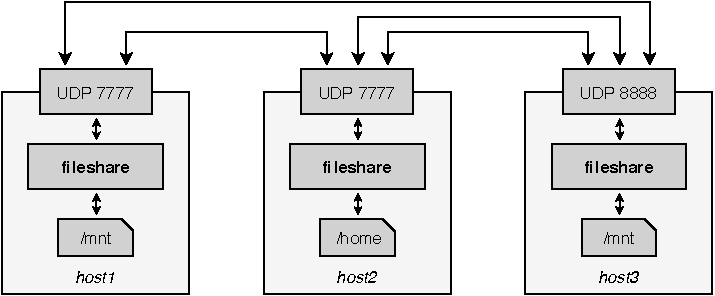
\includegraphics{figures/arch.pdf}
  \caption{Arquitetura \nonpt{peer-to-peer} do sistema \SYS.}
  \label{fig:func:arch}
  \vspace*{-.7\baselineskip}
\end{figure}

\itemizedpar{Aceitação de pedidos de transferência.}

Cada \nonpt{peer} define, com recurso a uma \nonpt{whitelist}, quais os \nonpt{peers} que podem ter acesso à sub-árvore local exportada, tanto para transferências de \nonpt{download} como de \nonpt{upload}. Esta \nonpt{whitelist} consiste num conjunto de intervalos de endereços IPv4 e IPv6 em notação CIDR. Ao se receber um pedido de transferência, este apenas é aceite se o endereço do \nonpt{peer} que realizou o pedido pertencer a algum dos intervalos de endereços na \nonpt{whitelist}.

\itemizedpar{Transferências de \nonpt{download}.}

Um \nonpt{peer} pode obter um ficheiro a partir de um ou mais outros \nonpt{peers} realizando uma transferência de \nonpt{download}. O utilizador deve especificar o caminho para o ficheiro a ser obtido (relativo às raizes das sub-árvores exportadas pelos \nonpt{peers} remotos) e os endereços dos \nonpt{peers} a partir dos quais o ficheiro deve ser transferido. Pode-se ainda especificar o caminho do ficheiro local resultante da transferência, caso não se deseje utilizar o mesmo caminho que o do ficheiro remoto.

Caso o utilizador indique que deve ser utilizado mais de um \nonpt{peer} remoto para se realizar a transferência, o ficheiro é dividido em segmentos de tamanho igual e cada segmento é obtido de um \nonpt{peer} distinto, em paralelo. Neste caso é também verificado que todos os \nonpt{peers} reportam o mesmo tamanho de ficheiro.

\itemizedpar{Transferências de \nonpt{upload}.}

Cada \nonpt{peer} pode também enviar um ficheiro para um ou mais outros \nonpt{peers} iniciando uma transferência de \nonpt{upload}. O utilizador especifica o caminho para o ficheiro a ser enviado (relativo à raiz da sub-árvore exportada pelo \nonpt{peer} local) e os endereços dos \nonpt{peers} para os quais o ficheiro deve ser transferido. É ainda possível indicar o caminho do ficheiro remoto resultante da transferência, ao invés de se utilizar o mesmo caminho que o do ficheiro local.

Caso o utilizador indique mais de um \nonpt{peer} remoto, o ficheiro é transmitido em paralelo e na sua totalidade para cada um dos \nonpt{peers}.

\itemizedpar{Transferências concorrentes.}

O sistema permite realizar qualquer número transferências em simultâneo entre qualquer par de \nonpt{peers}, incluindo combinações de transferências de \nonpt{download} e \nonpt{upload}. Cada \nonpt{peer} garante que o mesmo ficheiro não é modificado concorrentemente por mais de uma transferência, permitindo no entanto acessos de leitura simultâneos.

Nota-se também que, ao se receber um ficheiro (seja por se ter requerido uma transferência de \nonpt{download} ou por se servir um pedido de transferência de \nonpt{upload}), as alterações a esse ficheiro apenas são tornadas visíveis se a transferência for realizada com sucesso na sua totalidade. Em particular, se um ficheiro com o mesmo caminho já existir, este não é alterado caso a transferência falhe ou não termine com sucesso.

% ---------------------------------------------------------------------------- %

\subsection{Interface de linha de comandos}

O sistema \SYS é constituído por um único programa (ficheiro \path{fileshare.jar} no arquivo \ARQUIVO disponibilizado juntamente com este relatório), o qual permite iniciar um \nonpt{peer} local e executar transferências utilizando outros \nonpt{peers}. O programa disponibiliza uma interface de linha de comandos e tem a seguinte forma de invocação:

\begin{minted}{bash}
    fileshare [-a|--allow-all] [-p|--port <n>] <export_dir>
\end{minted}

O argumento \verb|<export_dir>| especifica a raiz da sub-árvore de sistema de ficheiros local a ser exportada pelo \nonpt{peer}, devendo ser um caminho para uma diretoria. As opções têm os seguintes significados:

\begin{itemize}

    \item \verb|-a| ou \verb|--allow-all| --- especifica que qualquer outro \nonpt{peer} pode realizar transferências utilizando o \nonpt{peer} local;
    
    \item \verb|-p <n>| ou \verb|--port <n>| --- especifica a porta UDP local que o \nonpt{peer} deve utilizar (se esta opção não for dada, a porta 7777 é selecionada).

\end{itemize}

O programa disponibiliza um \nonpt{prompt} interativo onde o utilizador pode introduzir comandos com o objetivo de realizar transferências de ficheiros entre \nonpt{peers}. Para executar o programa, recomenda-se a utilização do \nonpt{script} \path{fileshare.sh} (incluído também no arquivo \ARQUIVO), o qual expõe o mesmo modo de utilização mas adiciona funcionalidades de histórico de comandos ao \nonpt{prompt} interativo.

O \nonpt{prompt} interativo disponibiliza os seguintes comandos:

\newcommand{\comando}[1]{\textbf{\texttt{#1}}}

\newcommand{\comandodesc}[3]{%
  \begin{description}[style=nextline]%
  \item[\textbf{\texttt{#1 }\mintinline{bash}{#2}}]%
  #3%
  \end{description}%
  }

\comandodesc{exit}{}{Termina o \nonpt{peer} local e sai do \nonpt{prompt} interativo. Equivalente a fechar a \nonpt{stream} de \nonpt{standard input} através da combinação de teclas Ctrl+D.}

\comandodesc{whitelist-add}{<cidr_peers...>}{Adiciona os padrões de endereços em notação CIDR especificados (separados por espaços) à \nonpt{whitelist} de endereços de \nonpt{peers}.}

\comandodesc{whitelist-remove}{<cidr_peers...>}{Remove os padrões de endereços em notação CIDR especificados (separados por espaços) da \nonpt{whitelist} de endereços de \nonpt{peers}.}

\comandodesc{whitelist-all}{}{Adiciona os padrões \path{0.0.0.0/0} e \path{::/0} à \nonpt{whitelist} de endereços de \nonpt{peers}, permitindo que qualquer outro \nonpt{peer} realize transferências utilizando o \nonpt{peer} local. Equivalente a se especificar a opção \texttt{-a} ou \texttt{--allow-all} ao se invocar o programa.}

\comandodesc{whitelist-clear}{}{Remove todos os padrões de endereços da \nonpt{whitelist} de endereços de \nonpt{peers}.}

\comandodesc{get}{<remote_file> [as <local_file>] from <peers...>}{Realiza o \nonpt{download} do ficheiro com o caminho \texttt{<remote\_file>} a partir dos \nonpt{peers} com endereços \texttt{<peers...>} (separados por espaços), armazenando-o com o caminho \texttt{<local\_file>} (ou, se não especificado, com o caminho \texttt{<remote\_file>}). Se for dado mais de um \nonpt{peer}, a transferência é particionada e realizada em simultâneo a partir deles.}

\comandodesc{put}{<local_file> [as <remote_file>] to <peers...>}{Realiza o \nonpt{upload} do ficheiro com o caminho \texttt{<local\_file>} para os \nonpt{peers} com endereços \texttt{<peers...>} (separados por espaços), armazenando-o com o caminho \texttt{<remote\_file>} (ou, se não especificado, com o caminho \texttt{<local\_file>}). Se for dado mais de um \nonpt{peer}, a transferência é realizada em simultâneo para todos eles.}

\comandodesc{concurrent}{}{Permite realizar qualquer número e tipo de transferências em simultâneo. Execuções de \comando{get} e \comando{put} após a utilização deste comando apenas são realizadas ao se introduzir o comando \comando{run}, após o qual se regressa ao modo de execução imediata de transferências. O comando \comando{cancel} pode ser utlizado para se cancelar a realização de transferências já introduzidas e se voltar ao modo de execução imediata.}

% ---------------------------------------------------------------------------- %

\subsection{Exemplos de utilização}

Apresentam-se de seguida exemplos de utilização do programa \path{fileshare} e dos comandos do \nonpt{prompt} interativo disponibilizado pelo mesmo.

\begin{itemize}[noitemsep]

    \item Inicia um \emph{peer} na porta 8888, exportando a diretoria \path{/mnt}, e adiciona os intervalos de endereços \path{192.168.1.0/24} e \path{193.137.0.0/16} à \nonpt{whitelist}, ficando apto para servir transferências de ficheiros requeridas por \emph{peers} cujos endereços estejam contidos em algum de ambos esses intervalos.

    \vspace*{.9\baselineskip}
    \begin{Verbatim}[breaklines,gobble=8,frame=leftline,framesep=8pt,xleftmargin=11pt,commandchars=\\\{\}]
        \textcolor{Blue}{$} fileshare -p 8888 /mnt
        Exporting directory "/mnt" through UDP port 8888.
        \textcolor{RoyalBlue}{>} whitelist-add 192.168.1.0/24 193.137.0.0/16
        \textcolor{RoyalBlue}{>}
    \end{Verbatim}
    \vspace*{.9\baselineskip}

    \item Inicia um \nonpt{peer} na porta 7777, exportando a diretoria \path{/mnt}, e realiza o \nonpt{download} do ficheiro \path{file-1} a partir dos \nonpt{peers} com endereços \path{192.168.1.123}, \path{192.168.1.234} e \path{172.157.2.167}, e portas 7777, 12345 e 7777, respetivamente. No exemplo, a transferência está em progresso, tendo-se já recebido 63\% do ficheiro.

    \vspace*{.9\baselineskip}
    \begin{Verbatim}[breaklines,gobble=8,frame=leftline,framesep=8pt,xleftmargin=11pt,commandchars=\\\{\}]
        \textcolor{Blue}{$} fileshare /mnt
        Exporting directory "/mnt" through UDP port 7777.
        \textcolor{RoyalBlue}{>} get file-1 from 192.168.1.123 192.168.1.234:12345 172.157.2.167
        \textcolor{YellowOrange}{[ 63\%]} Getting file-1 from 3 peers... (9673.28 KiB/s)
    \end{Verbatim}
    \vspace*{.9\baselineskip}

    \item Inicia um \nonpt{peer} na porta 7777, exportando a diretoria \path{/mnt}, e realiza, concorrentemente, \inlineenum{1} o \nonpt{download} do ficheiro \path{file-2} a partir do \nonpt{peer} com \nonpt{hostname} \path{host123} e porta 8888, e \inlineenum{2} o \nonpt{upload} do ficheiro \path{my-things/file-3} para o \nonpt{peer} com \nonpt{hostname} \path{host123} e para o \nonpt{peer} com endereço \path{172.157.2.167}, ambos na porta 7777, e com o nome \path{another-name} nos \nonpt{peers} de destino. A primeira transferência falhou devido ao \nonpt{peer} remoto rejeitar a conecção (o endereço local não pertence à \nonpt{whitelist} desse \nonpt{peer}). A segunda transferência terminou com sucesso.

    \vspace*{.9\baselineskip}
    \begin{Verbatim}[breaklines,gobble=8,frame=leftline,framesep=8pt,xleftmargin=11pt,commandchars=\\\{\}]
        \textcolor{Blue}{$} fileshare /mnt
        Exporting directory "/mnt" through UDP port 7777.
        \textcolor{RoyalBlue}{>} concurrent
          \textcolor{RoyalBlue}{>} get file-2 from host123:8888
          \textcolor{RoyalBlue}{>} put my-things/file-3 as another-name to host123 172.157.2.167
          \textcolor{RoyalBlue}{>} run
          \textcolor{BrickRed}{ERROR!} The peer refused to establish a connection.
          \textcolor{ForestGreen}{[100\%]} Put file-1 to 2 peers. (23.74 MiB/s)
        \textcolor{RoyalBlue}{>} exit
        \textcolor{Blue}{$}
    \end{Verbatim}

\end{itemize}

% ---------------------------------------------------------------------------- %

% ---------------------------------------------------------------------------- %

\section{Implementação}
\label{sec:impl}

Tendo-se apresentado as funcionalidades disponibilizadas pelo sistema \SYS, descre\-ve-se nesta secção a implementação do mesmo, primeiro delineando a sua arquitetura e depois detalhando os seus principais componentes.

% ---------------------------------------------------------------------------- %

\subsection{Arquitetura}

O sistema foi integralmente implementado na linguagem Java (versão \emph{Java SE 11}), fazendo uso das duas bibliotecas seguintes:

\begin{itemize}

    \item \emph{argparse4j}\footnote{\url{https://argparse4j.github.io/}} versão 0.8.1, utilizada para processar os argumentos da linha de comandos;
    
    \item \emph{IPAddress}\footnote{\url{https://seancfoley.github.io/IPAddress/}} versão 5.0.2, utilizada para processar \nonpt{strings} em notação CIDR, representando intervalos contíguos de endereços IPv4 ou IPv6.
    
\end{itemize}

A implementação do sistema foi divida em três camadas, a cada uma correspondendo um \nonpt{package} Java:

\begin{enumerate}

    \item \emph{Camada de comunicação fiável} (\nonpt{package} \texttt{fileshare.transport}), encapsulando a implementação do protocolo de transferência fiável de dados sobre UDP e expondo uma interface de estabelecimento de conecções para comunicação entre \nonpt{hosts};

    \item \emph{Camada de transferência de ficheiros} (\nonpt{package} \texttt{fileshare.core}), utilizando a camada anterior para implementar toda a lógica de transferência de ficheiros entre \nonpt{peers};

    \item \emph{Camada de interface de utilizador} (\nonpt{package} \texttt{fileshare.ui}), implementando a interface de linha de comandos do programa, recorrendo a serviços expostos pela camada anterior.

\end{enumerate}

As interdependências entre estes três \nonpt{packages} é ilustrada na Figura~\ref{fig:impl:packages}. O código-fonte do sistema está extensivamente documentado através de comentários Javadoc embutidos no próprio código-fonte.

\begin{figure}[ht]
  \centering
  \vspace*{.3\baselineskip}
  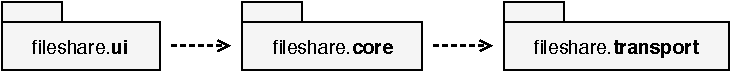
\includegraphics[scale=.9]{figures/packages.pdf}
  \caption{Dependências entre \nonpt{packages} Java da implementação do sistema.}
  \label{fig:impl:packages}
  \vspace*{.1\baselineskip}
\end{figure}

Em cada uma das subsecções seguintes, detalham-se os aspetos mais relevantes de cada uma das camadas supramencionadas, na ordem apresentada anteriormente.

% ---------------------------------------------------------------------------- %

\subsection{Camada de comunicação fiável}

A camada de comunicação fiável implementa um protocolo de comunicação sobre UDP com garantia de transmissão sem erros e de ordem. Apresenta-se aqui primeiro a interface exposta por esta camada, detalhando-se depois o funcionamento do protocolo na qual esta se baseia.

\itemizedpar{Interface disponibilizada.}

As classes que constituem a interface pública desta camada pertencem ao \nonpt{package} \texttt{fileshare.transport} e são ilustradas na Figura~\ref{fig:impl:classes-transport}, juntamente com as suas interdependências ao nível da interface.

\begin{figure}[ht]
  \centering
  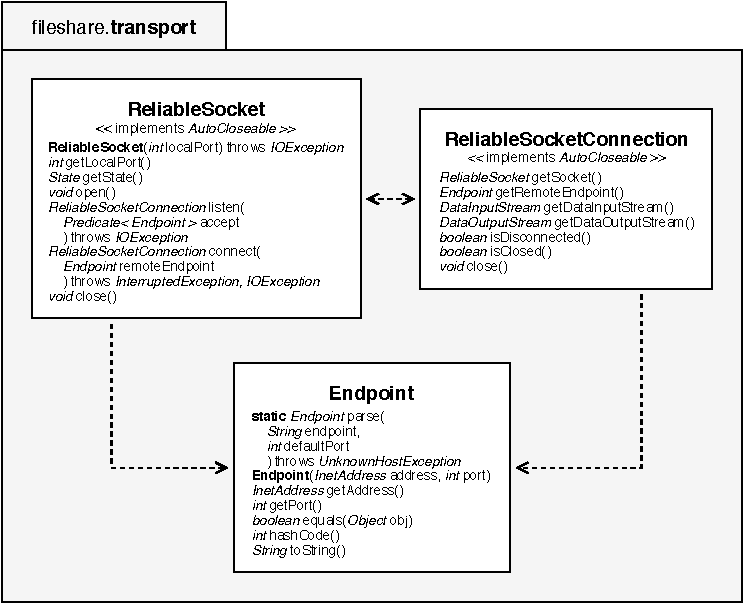
\includegraphics{figures/classes-transport.pdf}
  \caption{Classes do \emph{package} \texttt{fileshare.transport} e dependências ao nível da interface.}
  \label{fig:impl:classes-transport}
\end{figure}

A classe \texttt{Endpoint} representa um par endereço-porta, similarmente à classe \path{java.net.InetSocketAddress}. Ao contrário desta última, no entanto, a classe \texttt{Endpoint} não permite \nonpt{hostnames} não resolvidos, garantindo que erros relativos à resolução de nomes são tratados pelas camadas superiores.

A classe principal desta camada, \texttt{ReliableSocket}, gere um \nonpt{socket} UDP local, permitindo estabelecer conecções \nonpt{duplex} com outros \nonpt{sockets} similares, estas últimas sendo representadas por instâncias da classe \texttt{ReliableSocketConnection}.

O método \texttt{connect()} da classe \texttt{ReliableSocket} permite efetuar pedidos de establecimento de conecções com outros \nonpt{sockets}. O método \texttt{listen()} é utilizado para a tratar estes pedidos de conecção, permitindo também definir um predicado que determine se um dado pedido de conecção deve ser aceite ou rejeitado.

Os métodos \path{getDataInputStream()} e \path{getDataOutputStream()}, ambos da classe \path{ReliableSocketConnection}, devolvem \nonpt{streams} que podem ser utilizadas para se receber e enviar dados através da conecção respetiva. O método \path{close()} termina a conecção.

Para mais informações sobre a interface exposta por esta camada, remete-se o leitor para a documentação \nonpt{Javadoc} embutida no código-fonte.

\itemizedpar{Protocolo de comunicação fiável.}

A camada de comunicação fiável permite estabelecer canais \nonpt{duplex} de comunicação orientados à conecção, com garantia de transmissão sem erros, sem dados duplicados e ordenada. Todas as interações entre os \nonpt{sockets} descritos acima são, internamente, realizadas através de \nonpt{packets}, os quais podem ser de vários tipos, cada um tendo o seu formato específico. Estes tipos, significados correspondentes e formatos são especificados na Tabela~\ref{tbl:impl:tipos-packets}.

\begin{table}[ht]
  \centering
  \setlength{\tabcolsep}{6.5pt}
  \renewcommand{\arraystretch}{1.3}
  \begin{tabularx}{\textwidth}{|l|X|l|}
  
    \hline
    \multicolumn{1}{|c|}{\textbf{Tipo}} &
    \multicolumn{1}{c|}{\textbf{Descrição}} &
    \multicolumn{1}{c|}{\textbf{Formato}}
    \\ \hline
    
    \texttt{CONN}
     & \multirow[t]{3}{=}{Pedido de estabelecimento de conecção}
       & 4 bytes: Checksum \\
     & & 1 byte: Identificador do tipo de pacote (= 0) \\
     & & 2 bytes: Identificador local da conecção \\
    \hline
    
    \texttt{CONN-ACCEPT}
     & \multirow[t]{3}{=}{Notificação da aceitação de um pedido de conecção}
       & 4 bytes: Checksum \\
     & & 1 byte: Identificador do tipo de pacote (= 1) \\
     & & 2 bytes: Identificador remoto da conecção \\
     & & 2 bytes: Identificador local da conecção \\
    \hline

    \texttt{CONN-REJECT}
     & \multirow[t]{3}{=}{Notificação da rejeição de um pedido de conecção}
       & 4 bytes: Checksum \\
     & & 1 byte: Identificador do tipo de pacote (= 2) \\
     & & 2 bytes: Identificador remoto da conecção \\
    \hline
    
    \texttt{DATA}
     & \multirow[t]{3}{=}{Envio de dados}
       & 4 bytes: Checksum \\
     & & 1 byte: Identificador do tipo de pacote (= 3) \\
     & & 2 bytes: Identificador local da conecção \\
     & & 8 bytes: Posição dos dados na \emph{stream} \\
     & & Entre 1 e 1415 bytes: Dados (\emph{payload}) \\
    \hline
    
    \texttt{DATA-ACK}
     & \multirow[t]{3}{=}{Confirmação da receção de dados}
       & 4 bytes: Checksum \\
     & & 1 byte: Identificador do tipo de pacote (= 4) \\
     & & 2 bytes: Identificador local da conecção \\
     & & 8 bytes: Posição na \emph{stream} tal que todos os \\
     & & \hfill dados anteriores tenham sido recebidos \\
    \hline
    
    \texttt{DISC}
     & \multirow[t]{3}{=}{Notificação do término da conecção}
       & 4 bytes: Checksum \\
     & & 1 byte: Identificador do tipo de pacote (= 5) \\
     & & 2 bytes: Identificador local da conecção \\
    \hline
    
    \texttt{DISC-ACK}
     & \multirow[t]{3}{=}{Confirmação da receção da notificação do término da conecção}
       & 4 bytes: Checksum \\
     & & 1 byte: Identificador do tipo de pacote (= 6) \\
     & & 2 bytes: Identificador local da conecção \\
    \hline
    
  \end{tabularx}
  \caption{Tipos de \nonpt{packets} trocados pelo protocolo de comunicação fiável.}
  \label{tbl:impl:tipos-packets}
\end{table}

A descrição que se segue faz referência a vários valores não especificados, tais como \nonpt{timeouts} e números máximos de retransmissões. Estes valores estão definidos na classe \texttt{Config} do \nonpt{package} \texttt{fileshare.transport}.

Os primeiros 5 bytes de todos os \nonpt{packets} seguem o mesmo formato: 4 bytes para um \nonpt{checksum} e 1 byte para identificar o tipo de \nonpt{packet}. O \nonpt{checksum} é computado por quem envia o \nonpt{packet}, com base no conteúdo do mesmo, e é recomputado e comparado pelo destinatário. Se o \nonpt{checksum} recebido no \nonpt{packet} tiver um valor distinto do computado pelo recipiente, o \nonpt{packet} é simplesmente descartado.

Por forma a se estabelecer uma conecção, é enviado um \nonpt{packet} do tipo \texttt{CONN}. Ao receber um destes \nonpt{packets}, o recipiente responde com um outro \nonpt{packet} do tipo \texttt{CONN-ACCEPT} ou \texttt{CONN-REJECT}, aceitando ou rejeitando a conecção, respetivamente. Se o \nonpt{packet} \texttt{CONN} não obtiver resposta, este é reenviado (após um determinado intervalo de tempo). Se após um certo número de retransmissões não existir resposta, é reportado um erro à camada superior.

Após se estabelecer uma conecção, ambos os lados da conecção podem enviar dados através de \texttt{packets} do tipo \texttt{DATA}. O recipiente deve depois enviar um \nonpt{packet} \texttt{DATA-ACK} por forma a reconhecer a receção dos dados. Se não for recebido um \nonpt{packet} \texttt{DATA-ACK}, os dados são retransmitidos. Resumidamente, é seguida uma abordagem \emph{Go-Back-N}, não existem \nonpt{acknowledgments} negativos e os \nonpt{acknowledgments} são cumulativos e expressos como \nonpt{offsets} em bytes correspondentes aos dados recebidos desde que a conecção foi estabelecida.

Ao terminar uma conecção é enviado um \nonpt{packet} \texttt{DISC}, aguardando-se depois uma resposta na forma de um \nonpt{packet} \texttt{DISC-ACK}. O \nonpt{packet} \texttt{DISC} é retransmitido se não houver resposta, até um determinado número máximo de retransmissões, após o qual a conecção é considerada, de qualquer forma, terminada.

Se um dos lados da conecção morrer, isto é detetado pela ausência de respostas \texttt{DATA-ACK} a dados enviados, e a conecção é dada como terminada.

% ---------------------------------------------------------------------------- %

\subsection{Camada de transferência de ficheiros}

A camada de transferência de ficheiros implementa, com recurso à camada de comunicação fiável previamente descrita, o protocolo \nonpt{peer-to-peer} de transferência de ficheiros disponibilizado pelo sistema \SYS. De seguida apresenta-se a interface exposta por esta camada, descrevendo-se também os protocolos de comunicação entre \nonpt{peers} para a execução de transferências de ficheiros.

\itemizedpar{Interface disponibilizada.}

As classes que constituem a interface pública da camada de transferência de ficheiros, todas pertencentes ao \nonpt{package} \path{fileshare.core}, são ilustradas na Figura~\ref{fig:impl:classes-core} juntamente com as suas interdependências ao nível da interface.

\begin{figure}[p]
  \centering
  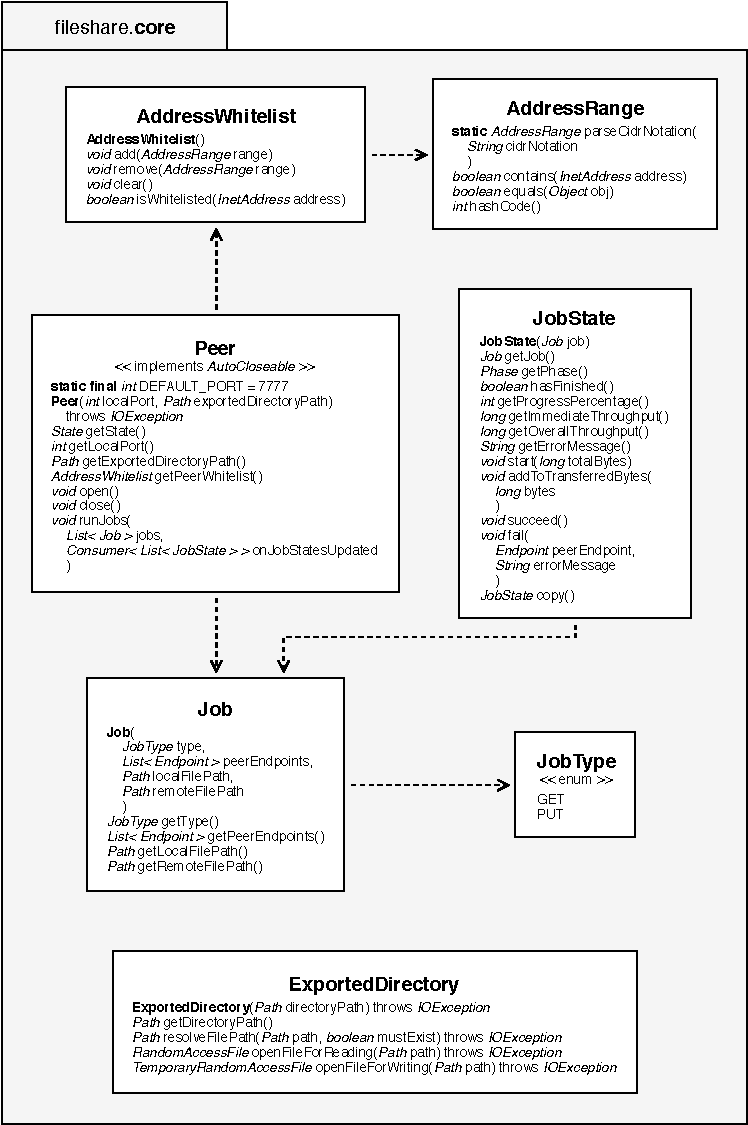
\includegraphics{figures/classes-core.pdf}
  \caption{Classes do \emph{package} \texttt{fileshare.core} e dependências ao nível da interface.}
  \label{fig:impl:classes-core}
\end{figure}

A classe \texttt{Peer} gere um \nonpt{peer} local no sistema \SYS, sendo então a classe central desta camada. A sua interface permite gerir a \nonpt{whitelist} de endereços de \nonpt{peers}, descrita previamente, e, através do método \texttt{runJobs()}, iniciar a execução de transferências de ficheiros --- aqui denominadas de \emph{jobs} --- com outros \nonpt{peers}. Esta classe serve também, em segundo plano, pedidos de transferência de ficheiros realizados por outros \nonpt{peers}.

Brevemente, as restantes classes e enumerações têm as seguintes responsabilidades:

\begin{itemize}
    \item \texttt{AddressRange} -- representa um intervalo contíguo de endereços IPv4 ou IPv6;
    \item \texttt{AddressWhitelist} -- utilizada para representar a \nonpt{whitelist} de endereos de \nonpt{peers};
    \item \texttt{ExportedDirectory} -- gere a sub-árvore do sistema de ficheiros exportada pelo \nonpt{peer};
    \item \texttt{JobType} -- define os dois tipos de transferência: \nonpt{download} (\texttt{GET}) e \nonpt{upload} (\texttt{PUT});
    \item \texttt{Job} -- define uma transferência de um ficheiro, em qualquer direção e envolvendo qualquer número de \nonpt{peers} remotos;
    \item \texttt{JobState} -- representa o estado de um \nonpt{job} que está a decorrer.
\end{itemize}

Para mais informações sobre a interface exposta por esta camada, remete-se o leitor para a documentação \nonpt{Javadoc} embutida no código-fonte.

\itemizedpar{Protocolo de transferência de ficheiros.}

Para executar um \nonpt{job}, o \nonpt{peer} estabelece conecções com todos os outros \nonpt{peers} envolvidos na transferência e segue, depois, um protocolo de comunicação específico à direção da transferência.

Os protocolos utilizados em transferências dos tipos \emph{get} e \emph{put} são delineados nas Tabelas~\ref{tbl:impl:protocolo-get} e~\ref{tbl:impl:protocolo-put}, respetivamente, onde o \emph{cliente} corresponde ao \nonpt{peer} que requeriu a transferência e o \emph{servidor} corresponde ao \nonpt{peer} restante (caso exista mais de um \nonpt{peer} remoto, o protocolo é seguido para cada um deles). Explicita-se que estas tabelas não são uma especificação completa do protocolo, em particular não apresentando todos os casos de erro, destinando-se apenas a ilustrar a implementação do mesmo.

\begin{table}[p]
    \centering
    \setlength{\tabcolsep}{6.5pt}
    \renewcommand{\arraystretch}{1.15}
    \begin{tabularx}{\textwidth}{|p{2cm}|X|X|}
        \cline{2-3}
        \multicolumn{1}{l|}{} & \multicolumn{1}{c|}{\textbf{Cliente}} & \multicolumn{1}{c|}{\textbf{Servidor}} \\
        \hline \multirow[t]{5}{=}{Comportamento normal}
         & \verb|writeByte(0)| (tipo de \emph{job}) & \\
         & \verb|writeUTF(path_file_servidor)| & \\
         & \verb|flush()| & \\
         & & \verb|readByte()| (= 0) \\
         & & \verb|path_file_servidor = readUTF()| \\
         & & [se erro, ir para \emph{caso de erro 1}] \\
         & & \verb|writeLong(tamanho_file)| \\
         & & \verb|flush()| \\
         & \verb|tamanho_file = readLong()| & \\
         & [se erro, ir para \emph{caso de erro 2}] & \\
         & \verb|writeLong(offset_segmento)| & \\
         & \verb|writeLong(tamanho_segmento)| & \\
         & \verb|flush()| & \\
         & & \verb|offset_segmento = readLong()| \\
         & & \verb|tamanho_segmento = readLong()| \\
         & & escreve conteúdo do segmento \\
         & & \verb|flush()| \\
         & & \verb|close()| \\
         & lê e armazena conteúdo do segmento & \\
         & \verb|close()| & \\
        \hline \multirow[t]{5}{=}{Caso de erro 1 (\emph{e.g.}, ficheiro não existe no servidor)}
         & & \verb|writeLong(-1)| \\
         & & \verb|writeUTF(mensagem_erro)| \\
         & & \verb|flush()| \\
         & & \verb|close()| \\
         & \verb|readLong()| (= -1) & \\
         & \verb|mensagem_erro = readUTF()| & \\
         & reporta erro & \\
         & \verb|close()| & \\
        \hline \multirow[t]{5}{=}{Caso de erro 2 (\emph{e.g.}, tamanhos distintos entre servidores)}
         & reporta erro & \\
         & \verb|close()| & \\
         & & deteta \emph{end-of-file} \\
         & & \verb|close()| \\
        \hline
    \end{tabularx}
    \caption{Protocolo de comunicação entre dois \emph{peers}, ao nível da camada de transferência de ficheiros, para execução de um \emph{job} do tipo \emph{get}.}
    \label{tbl:impl:protocolo-get}
\end{table}

\begin{table}[p]
    \centering
    \setlength{\tabcolsep}{6.5pt}
    \renewcommand{\arraystretch}{1.15}
    \begin{tabularx}{\textwidth}{|p{2cm}|X|X|}
        \cline{2-3}
        \multicolumn{1}{l|}{} & \multicolumn{1}{c|}{\textbf{Cliente}} & \multicolumn{1}{c|}{\textbf{Servidor}} \\
        \hline \multirow[t]{5}{=}{Comportamento normal}
         & \verb|writeByte(1)| (tipo de \emph{job}) & \\
         & \verb|writeUTF(path_file_servidor)| & \\
         & \verb|writeLong(tamanho_file)| & \\
         & \verb|flush()| & \\
         & & \verb|readByte()| (= 1) \\
         & & \verb|path_file_servidor = readUTF()| \\
         & & \verb|tamanho_file = readLong()| \\
         & & [se erro, ir para \emph{caso de erro 1}] \\
         & & \verb|writeUTF("")| \\
         & & \verb|flush()| \\
         & \verb|readUTF()| (= \verb|""|) & \\
         & escreve conteúdo do ficheiro & \\
         & \verb|flush()| & \\
         & & lê e armazena conteúdo do ficheiro \\
         & & [se erro, ir para \emph{caso de erro 2}] \\
         & & \verb|writeUTF("")| \\
         & & \verb|flush()| \\
         & & \verb|close()| \\
         & \verb|readUTF()| (= \verb|""|) & \\
         & \verb|close()| & \\
        \hline \multirow[t]{5}{=}{Caso de erro 1 (\emph{e.g.}, ficheiro está em utilização)}
         & & \verb|writeUTF(mensagem_erro)| \\
         & & \verb|flush()| \\
         & & \verb|close()| \\
         & \verb|mensagem_erro = readUTF()| & \\
         & \verb|close()| & \\
         & reporta erro & \\
        \hline \multirow[t]{5}{=}{Caso de erro 2 (\emph{e.g.}, erro ao escrever ficheiro)}
         & & \verb|writeUTF(mensagem_erro)| \\
         & & \verb|flush()| \\
         & & \verb|close()| \\
         & \verb|mensagem_erro = readUTF()| & \\
         & \verb|close()| & \\
         & reporta erro & \\
        \hline
    \end{tabularx}
    \caption{Protocolo de comunicação entre dois \emph{peers}, ao nível da camada de transferência de ficheiros, para execução de um \emph{job} do tipo \emph{put}.}
    \label{tbl:impl:protocolo-put}
\end{table}

% ---------------------------------------------------------------------------- %

\subsection{Camada de interface de utilizador}

Por fim, a camada de interface de utilizador implementa a interface de linha de comandos disponibilizada pelo comando \path{fileshare}. Para efeitos de referência, as classes que implementam esta camada são ilustradas na Figura~\ref{fig:impl:classes-ui}. No entanto, considera-se que a descrição detalhada desta camada está fora do âmbito do presente relatório.

Como tal, para mais informações sobre a implementação desta camada, remete-se o leitor para a documentação \emph{Javadoc} embutida no código-fonte.

\begin{figure}[ht]
  \centering
  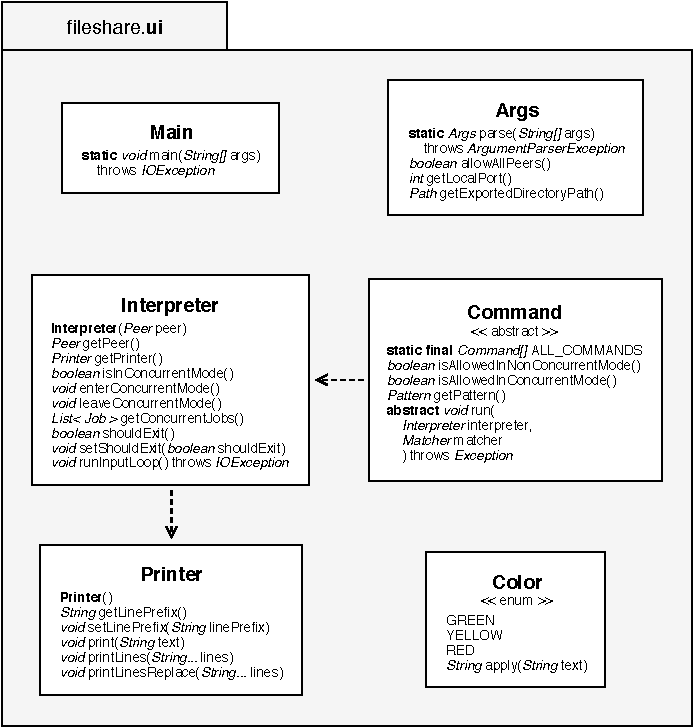
\includegraphics{figures/classes-ui.pdf}
  \caption{Classes do \emph{package} \texttt{fileshare.ui} e dependências ao nível da interface.}
  \label{fig:impl:classes-ui}
\end{figure}

% ---------------------------------------------------------------------------- %

% ---------------------------------------------------------------------------- %

\section{Conclusão}
\label{sec:conclusao}

Este relatório apresentou uma resolução ao terceiro trabalho prático desenvolvido no âmbito da Unidade Curricular de Comunicações por Computador do curso de Mestrado Integrado em Engenharia Informática, no ano letivo de 2018/2019, da Universidade do Minho.

Com este trabalho estudaram-se o modo de utilização e os mecanismos de funcionamento do serviço DNS de resolução de nomes. Todas as questões propostas pelo enunciado do trabalho foram respondidas. A criação e configuração do domínio de nomes \path{CC.PT} foi também realizada e todos os requisitos identificados pelo enunciado foram cumpridos.

% ---------------------------------------------------------------------------- %


\end{document}

% ---------------------------------------------------------------------------- %
